\documentclass{beamer}
\usepackage[english]{layout}
\usepackage[utf8]{inputenc}
\usepackage[english]{babel}
\usepackage[T1]{fontenc}
\usepackage{amsmath, soul, color, multicol, type1cm, verbatim, latexsym, dsfont, float, listings,alltt}
\usepackage[official]{eurosym}
\usepackage{beamerthemesplit}
\usetheme{Frankfurt}
\usecolortheme{lily}
%\usefonttheme{structuresmallcapsserif}
\usefonttheme{professionalfonts}
\setbeamercovered{transparent}

%NeSI Colors <---------------------------------------------------------------------------------------
\usecolortheme[RGB={47, 68, 71}]{structure} 
\definecolor{nesidark}{HTML}{2F4447}
\definecolor{nesilight}{HTML}{CED9DF}
\definecolor{nesigrey}{gray}{0.7}
\definecolor{nesilightgrey}{gray}{0.98}
\definecolor{nesidarkgrey}{gray}{0.3}
\definecolor{nesiblue}{HTML}{2B9FC2}
\setbeamercolor{block title}{fg=black,bg=nesigrey}
\setbeamercolor{block body}{bg=nesilightgrey,fg=nesidarkgrey}
\setbeamercolor{block body alerted}{bg=white,fg=black}
\setbeamercolor{alerted text}{bg=white,fg=black}

\setbeamerfont{title}{size=\huge}
\frenchspacing
\hyphenation{NeSI}

\newcommand\BackgroundPicture[1]{%
\setbeamertemplate{background}{%
\parbox[c][\paperheight]{\paperwidth}{%
\vfill \hfill \includegraphics[height=0.9\paperheight]{#1}
\hfill \vfill
}}}

\setbeamertemplate{blocks}[default]%[shadow=false]
\useinnertheme{circles}
\setbeamertemplate{title page}[default][center,rounded=false,shadow=false]

\title{Introduction to Intel Xeon Phi Workshop}
\subtitle{Computational Science Team @ NeSI}
\author{Jordi Blasco \\(jordi.blasco@nesi.org.nz)}
\date{}


\begin{document}

{
\setbeamertemplate{background canvas}{
\includegraphics[height=0.99\paperheight]{NeSI_img/Slide00.png}} 
\begin{frame}[plain]
\vspace{1cm}
\titlepage
\end{frame}
}


%\BackgroundPicture{NeSI_img/SlideXX.png}
\begin{frame}
\frametitle{Outline}
\begin{multicols}{2}
   \tableofcontents
 \end{multicols}
 \end{frame}


%%%%%%%%%%%%%%%%%%%%%%%%%%%%%%%%%%%%%%%%%%%%%%%%%%%%%%%%%%%%%%%%%%%%%%%%%%%%%%%%%%%%%%%%%%%%%%%
%%%%%%%%%%%%%%%%%%%%%%%%%%%%%%%%%%%%%%%%%%%%%%%%%%%%%%%%%%%%%%%%%%%%%%%%%%%%%%%%%%%%%%%%%%%%%%%



\section{Intel Xeon Phi overview}
\subsection{Why this enthusiasm with Intel Phi?}
\frame[t]
{
  \frametitle{Intel Xeon Phi co-processor overview}
 \begin{block}{Why this enthusiasm about Intel Phi?}
   \begin{itemize}%[<+-| alert@+>]
	\item You don't need to learn a new programming language (CUDA,…)
	\item You don't need to change the code in order to run on MIC.
	\item But,….
	\item The Intel MIC CPUs are slow comparing with the current Xeon.
	\item To get real performance you need to apply some changes.
	\item Is not easy, but a medium size code can be modified in few hours or days.
	\item Comparing with other architectures, it's like child's play.
   \end{itemize}
  \end{block}
}

\frame[t]
{
  \frametitle{Intel Xeon Phi co-processor overview}
    %  \begin{block}{Top application list}
    \begin{figure}
         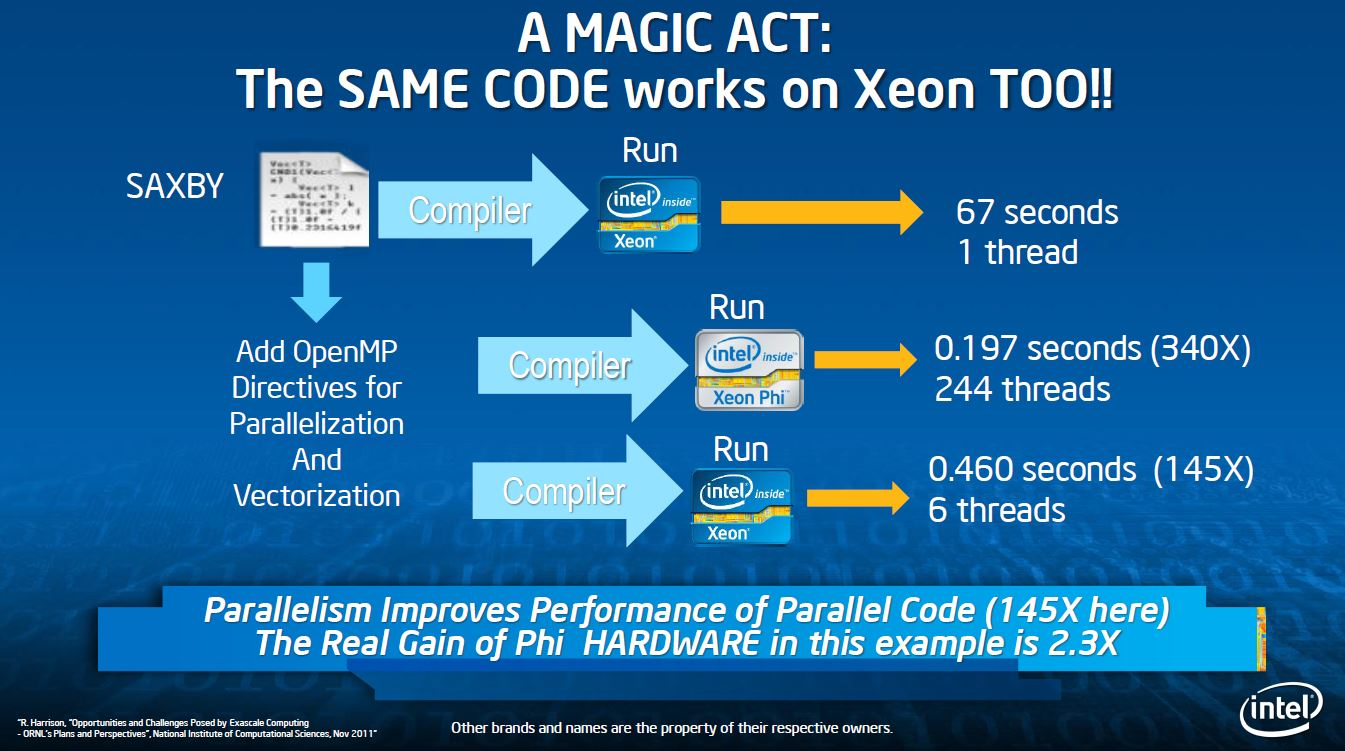
\includegraphics[width=\textwidth]{NeSI_img/intel-xeon-phi-carte-calcul.jpg}
         \caption{source www.intel.com}
    \end{figure}   
  %\end{block}
}

\frame[t]
{
  \frametitle{Intel Xeon Phi co-processor overview}
    %  \begin{block}{Top application list}
    \begin{figure}
         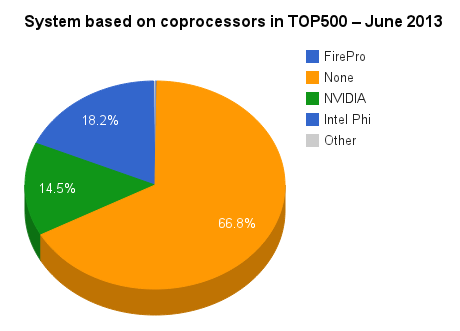
\includegraphics[width=0.8\textwidth]{NeSI_img/accelerators-t500june2013.png}
         \caption{source Top500 http://www.top500.org/statistics/list/}
    \end{figure}   
  %\end{block}
}

\frame[t]
{
  \frametitle{Intel Xeon Phi co-processor overview}
    %  \begin{block}{Top application list}
    \begin{figure}
         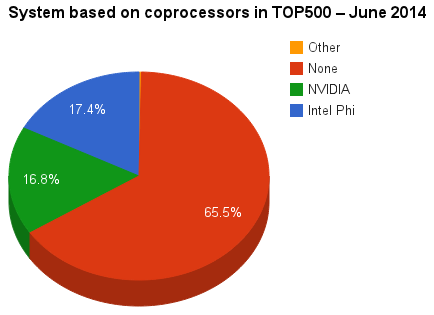
\includegraphics[width=0.8\textwidth]{NeSI_img/accelerators-t500june2014.png}
         \caption{source Top500 http://www.top500.org/statistics/list/}
    \end{figure}   
  %\end{block}
}

\subsection{Hardware specs}
\frame[t]
{
  \frametitle{Hardware specs}
   \begin{block}{Hardware specs of 5110P (KNF)}
\begin{columns}[onlytextwidth]
  \begin{column}{0.3\textwidth}
  \begin{figure}
         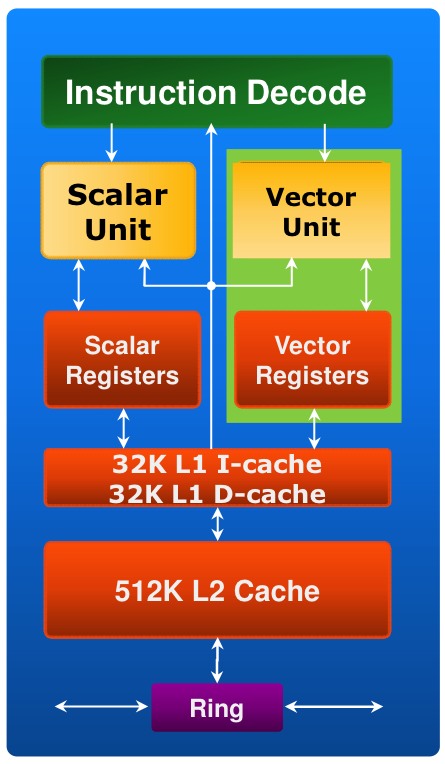
\includegraphics[width=\textwidth]{NeSI_img/mic-instruction-decode.png}
         %\caption{source www.intel.com}
  \end{figure}  
  \end{column}
  \begin{column}{0.7\textwidth}
  %\vspace{-0.8cm}
   \begin{itemize}%[<+-| alert@+>]
	\item 60 cores/1.053 GHz/240 threads.
	\item 30MB cache
	\item 8 GB memory and 320 GB/s bandwidth.
	\item GDDR5 x16 channels (5.5Gbit each).
	\item 300 ns access!
	\item Linux operating system, IP addressable.
	\item Built using Intel's 22nm process technology.
	\item 512-bit Single Instruction, Multiple Data instructions (SIMD).
	\item 32 vector registers.
   \end{itemize}
  \end{column}
\end{columns}
  \end{block}
}

\subsection{Roadmap}

\frame[t]
{
  \frametitle{Intel Xeon Phi Public Roadmap}
    %  \begin{block}{Top application list}
    \begin{figure}
         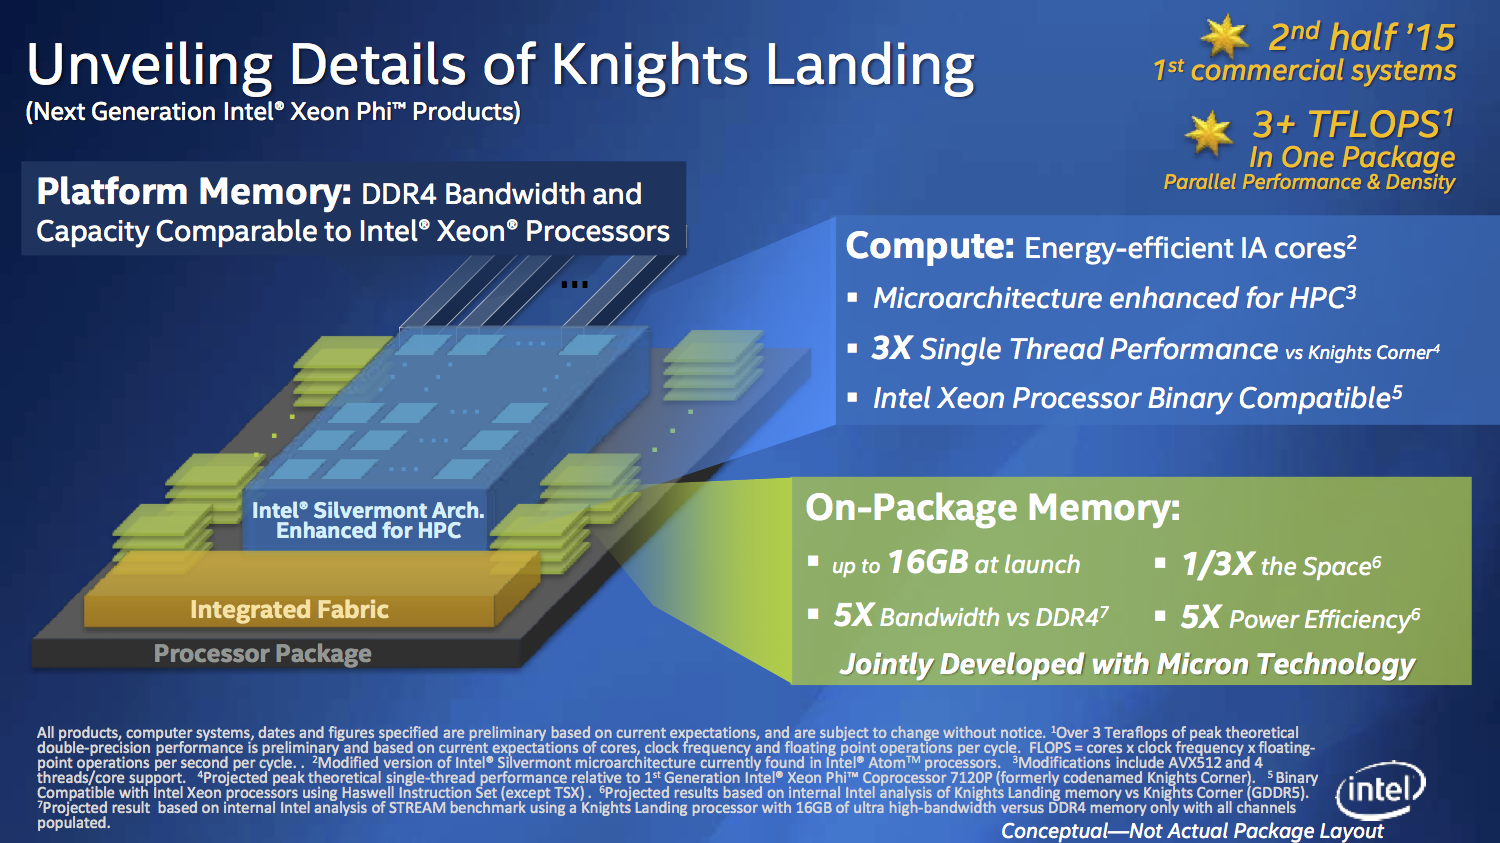
\includegraphics[width=\textwidth]{NeSI_img/KNL-features.png}
         \caption{source \url{http://newsroom.intel.com/servlet/JiveServlet/download/38-32805/ISC14_Raj_Hazra_keynote.pdf}}
    \end{figure}   
  %\end{block}
}

\frame[t]
{
  \frametitle{Intel Omni Scale Fabric Roadmap}
    %  \begin{block}{Top application list}
    \begin{figure}
         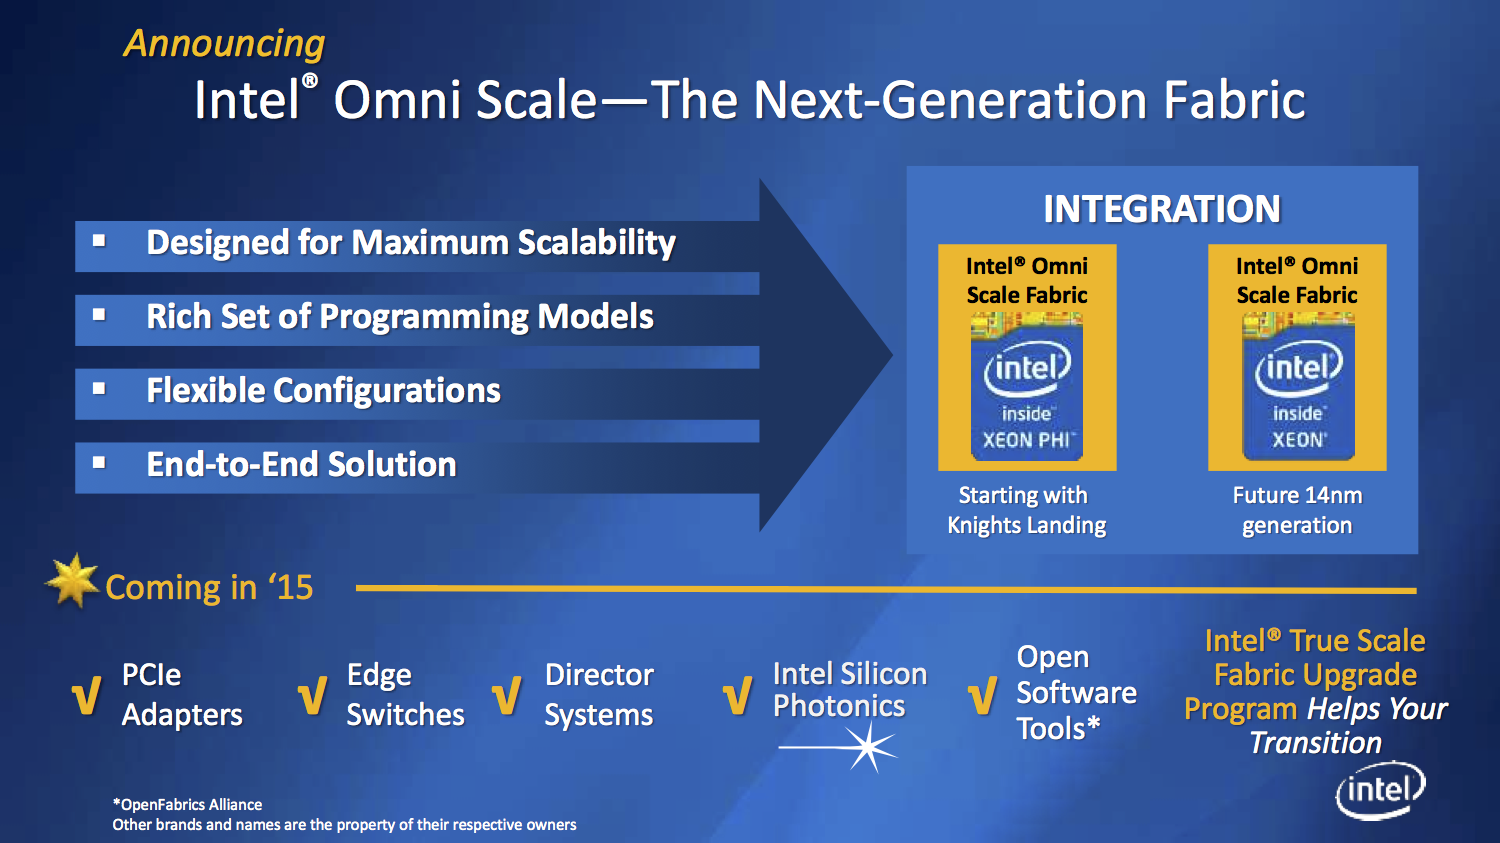
\includegraphics[width=\textwidth]{NeSI_img/intel-omni-scale-roadmap.png}
         \caption{source \url{http://newsroom.intel.com/servlet/JiveServlet/download/38-32805/ISC14_Raj_Hazra_keynote.pdf}}
    \end{figure}   
  %\end{block}
}

\frame[t]
{
  \frametitle{}
 \begin{block}{Matrix addition processing in scalar and vector mode.}
   \begin{itemize}%[<+-| alert@+>]
	\item \textbf{SSE} 128-bit (streaming) SIMD / 4 elements at a time (2008).
	\item \textbf{AVX} 256-bit SIMD / 8 elements at a time (2011).
	\item \textbf{MIC} 512-bit SIMD / 16 elements at  a time (2012).
	\item \textbf{AVX3} 512-bit SIMD / 16 elements at  a time (2014).
   \end{itemize}
       \begin{figure}
         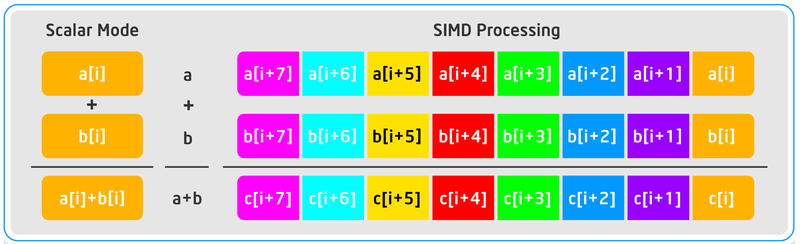
\includegraphics[width=\textwidth]{NeSI_img/simd_addition.png}
         \caption{source: www.intel.com}
    \end{figure}  
  \end{block}
}

\section{Parallel Strategies}
\subsection{How easy is it?}

\frame[t]
{
  \frametitle{Parallel Strategies}
% \begin{block}{}
    \begin{figure}
         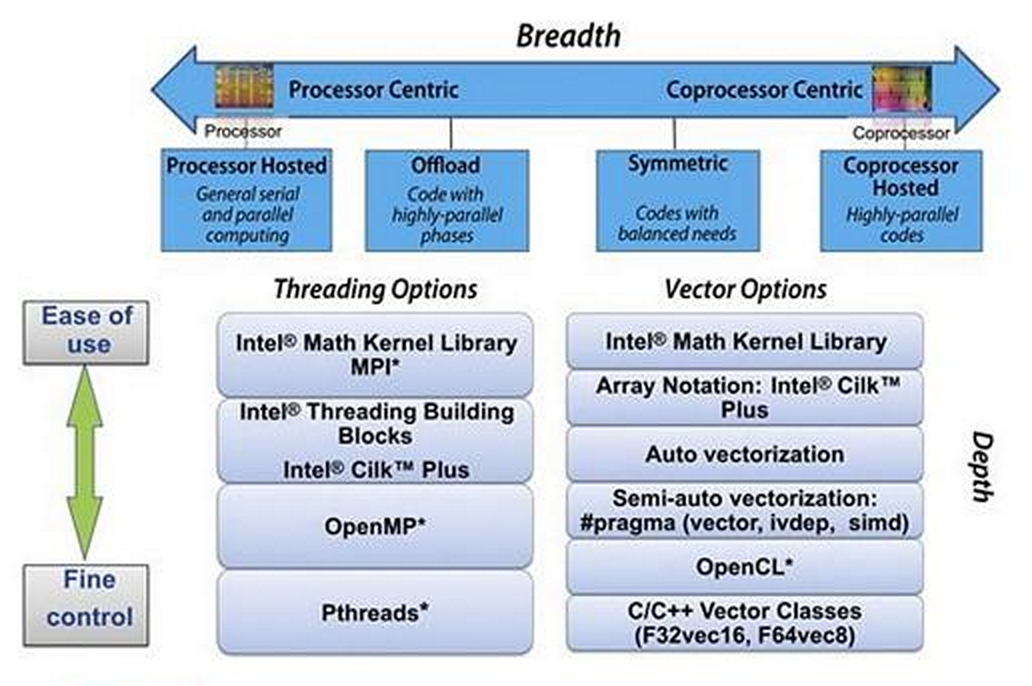
\includegraphics[width=0.9\textwidth]{NeSI_img/breadth-intel-phi.png}
         \caption{source www.intel.com}
    \end{figure}   
  %\end{block}
}

%\subsection{Programming Models}
%
%\frame[t]
%{
%  \frametitle{}
% \begin{block}{}
%   \begin{itemize}%[<+-| alert@+>]
%	\item 
%   \end{itemize}
%  \end{block}
%}

\subsection{Perfect Candidates}
\frame[t]
{
  \frametitle{Perfect Candidates}
 \begin{block}{Perfect Candidates}
   \begin{itemize}%[<+-| alert@+>]
	\item Serial applications that need to be run many times.
	\item Massive parallel applications (OpenMP).
	\item Massive parallel applications (MPI).
	\item Massive hybrid parallel applications (MPI+OpenMP).
	\item Applications that can exploit the vectorial capabilities of MIC.
   \end{itemize}
  \end{block}
}

\subsection{How to get the maximum performance on Intel Phi}

\frame[t]
{
  \frametitle{How to get the maximum performance on Intel Phi}
 \begin{block}{Maximize the performance in the processor first!}
   \begin{itemize}%[<+-| alert@+>]
	\item The first advise is to focus in the processor performance
	\item Audit the loops and find the hot-spots
	\item Profile the code
	\item Profile the MPI collectives
	\item Explore the Vectorization opportunities 
   \end{itemize}
  \end{block}
}


{
\setbeamertemplate{background canvas}{
\includegraphics[height=0.99\paperheight]{NeSI_img/Slide00.png}} 
\begin{frame}[plain]
\begin{center}
{\Huge Questions \& Answers}
\end{center}
\end{frame}
}


\frame[t]
{
  \frametitle{for more info}
 \begin{block}{Books}
   \begin{itemize}%[<+-| alert@+>]
	\item James Jeffers \& James Reinders, Intel Xeon Phi Coprocessor High Performance Programming, Newnes, 2013. ISBN: 0124104940
	\item James Reinders, Parallel Programming and Optimization with Intel® Xeon Phi™Coprocessors, Colfax 2013. ISBN-13: 978-0-9885234-1-8
   \end{itemize}
  \end{block}
   \begin{block}{Intel website (trainings and workshops)}
   \begin{itemize}%[<+-| alert@+>]
	\item \url{http://software.intel.com/en-us/mic-developer}
	\item \url{http://software.intel.com/en-us/intel-mkl}
	\item \url{http://software.intel.com/en-us/intel-composer-xe/}
   \end{itemize}
  \end{block}
}


\end{document}